\documentclass[twoside]{book}

% Packages required by doxygen
\usepackage{calc}
\usepackage{doxygen}
\usepackage{graphicx}
\usepackage[utf8]{inputenc}
\usepackage{makeidx}
\usepackage{multicol}
\usepackage{multirow}
\usepackage{textcomp}
\usepackage[table]{xcolor}

% Font selection
\usepackage[T1]{fontenc}
\usepackage{mathptmx}
\usepackage[scaled=.90]{helvet}
\usepackage{courier}
\usepackage{amssymb}
\usepackage{sectsty}
\renewcommand{\familydefault}{\sfdefault}
\allsectionsfont{%
  \fontseries{bc}\selectfont%
  \color{darkgray}%
}
\renewcommand{\DoxyLabelFont}{%
  \fontseries{bc}\selectfont%
  \color{darkgray}%
}

% Page & text layout
\usepackage{geometry}
\geometry{%
  a4paper,%
  top=2.5cm,%
  bottom=2.5cm,%
  left=2.5cm,%
  right=2.5cm%
}
\tolerance=750
\hfuzz=15pt
\hbadness=750
\setlength{\emergencystretch}{15pt}
\setlength{\parindent}{0cm}
\setlength{\parskip}{0.2cm}
\makeatletter
\renewcommand{\paragraph}{%
  \@startsection{paragraph}{4}{0ex}{-1.0ex}{1.0ex}{%
    \normalfont\normalsize\bfseries\SS@parafont%
  }%
}
\renewcommand{\subparagraph}{%
  \@startsection{subparagraph}{5}{0ex}{-1.0ex}{1.0ex}{%
    \normalfont\normalsize\bfseries\SS@subparafont%
  }%
}
\makeatother

% Headers & footers
\usepackage{fancyhdr}
\pagestyle{fancyplain}
\fancyhead[LE]{\fancyplain{}{\bfseries\thepage}}
\fancyhead[CE]{\fancyplain{}{}}
\fancyhead[RE]{\fancyplain{}{\bfseries\leftmark}}
\fancyhead[LO]{\fancyplain{}{\bfseries\rightmark}}
\fancyhead[CO]{\fancyplain{}{}}
\fancyhead[RO]{\fancyplain{}{\bfseries\thepage}}
\fancyfoot[LE]{\fancyplain{}{}}
\fancyfoot[CE]{\fancyplain{}{}}
\fancyfoot[RE]{\fancyplain{}{\bfseries\scriptsize Generated on Fri Apr 22 2016 22\-:51\-:08 for My Project by Doxygen }}
\fancyfoot[LO]{\fancyplain{}{\bfseries\scriptsize Generated on Fri Apr 22 2016 22\-:51\-:08 for My Project by Doxygen }}
\fancyfoot[CO]{\fancyplain{}{}}
\fancyfoot[RO]{\fancyplain{}{}}
\renewcommand{\footrulewidth}{0.4pt}
\renewcommand{\chaptermark}[1]{%
  \markboth{#1}{}%
}
\renewcommand{\sectionmark}[1]{%
  \markright{\thesection\ #1}%
}

% Indices & bibliography
\usepackage{natbib}
\usepackage[titles]{tocloft}
\setcounter{tocdepth}{3}
\setcounter{secnumdepth}{5}
\makeindex

% Hyperlinks (required, but should be loaded last)
\usepackage{ifpdf}
\ifpdf
  \usepackage[pdftex,pagebackref=true]{hyperref}
\else
  \usepackage[ps2pdf,pagebackref=true]{hyperref}
\fi
\hypersetup{%
  colorlinks=true,%
  linkcolor=blue,%
  citecolor=blue,%
  unicode%
}

% Custom commands
\newcommand{\clearemptydoublepage}{%
  \newpage{\pagestyle{empty}\cleardoublepage}%
}


%===== C O N T E N T S =====

\begin{document}

% Titlepage & ToC
\hypersetup{pageanchor=false}
\pagenumbering{roman}
\begin{titlepage}
\vspace*{7cm}
\begin{center}%
{\Large My Project }\\
\vspace*{1cm}
{\large Generated by Doxygen 1.8.6}\\
\vspace*{0.5cm}
{\small Fri Apr 22 2016 22:51:08}\\
\end{center}
\end{titlepage}
\clearemptydoublepage
\tableofcontents
\clearemptydoublepage
\pagenumbering{arabic}
\hypersetup{pageanchor=true}

%--- Begin generated contents ---
\chapter{Hierarchical Index}
\section{Class Hierarchy}
This inheritance list is sorted roughly, but not completely, alphabetically\-:\begin{DoxyCompactList}
\item \contentsline{section}{Binding}{\pageref{classBinding}}{}
\item \contentsline{section}{Cell}{\pageref{classCell}}{}
\item \contentsline{section}{Env\-Block}{\pageref{classEnvBlock}}{}
\item \contentsline{section}{Environment}{\pageref{classEnvironment}}{}
\item \contentsline{section}{Frame}{\pageref{classFrame}}{}
\item runtime\-\_\-error\begin{DoxyCompactList}
\item \contentsline{section}{Continue\-\_\-\-Directive}{\pageref{classContinue__Directive}}{}
\item \contentsline{section}{Evaluation\-\_\-\-Exception}{\pageref{classEvaluation__Exception}}{}
\item \contentsline{section}{No\-\_\-\-Binding\-\_\-\-Exception}{\pageref{classNo__Binding__Exception}}{}
\item \contentsline{section}{Not\-\_\-\-Subr}{\pageref{classNot__Subr}}{}
\item \contentsline{section}{Zipping\-\_\-\-Exception}{\pageref{classZipping__Exception}}{}
\end{DoxyCompactList}
\item \contentsline{section}{yy\-\_\-buffer\-\_\-state}{\pageref{structyy__buffer__state}}{}
\item \contentsline{section}{yy\-\_\-trans\-\_\-info}{\pageref{structyy__trans__info}}{}
\item \contentsline{section}{yyalloc}{\pageref{unionyyalloc}}{}
\item \contentsline{section}{Y\-Y\-S\-T\-Y\-P\-E}{\pageref{unionYYSTYPE}}{}
\end{DoxyCompactList}

\chapter{Class Index}
\section{Class List}
Here are the classes, structs, unions and interfaces with brief descriptions\-:\begin{DoxyCompactList}
\item\contentsline{section}{\hyperlink{classBinding}{Binding} }{\pageref{classBinding}}{}
\item\contentsline{section}{\hyperlink{classCell}{Cell} }{\pageref{classCell}}{}
\item\contentsline{section}{\hyperlink{classContinue__Directive}{Continue\-\_\-\-Directive} }{\pageref{classContinue__Directive}}{}
\item\contentsline{section}{\hyperlink{classEnvBlock}{Env\-Block} }{\pageref{classEnvBlock}}{}
\item\contentsline{section}{\hyperlink{classEnvironment}{Environment} }{\pageref{classEnvironment}}{}
\item\contentsline{section}{\hyperlink{classEvaluation__Exception}{Evaluation\-\_\-\-Exception} }{\pageref{classEvaluation__Exception}}{}
\item\contentsline{section}{\hyperlink{classFrame}{Frame} }{\pageref{classFrame}}{}
\item\contentsline{section}{\hyperlink{classNo__Binding__Exception}{No\-\_\-\-Binding\-\_\-\-Exception} }{\pageref{classNo__Binding__Exception}}{}
\item\contentsline{section}{\hyperlink{classNot__Subr}{Not\-\_\-\-Subr} }{\pageref{classNot__Subr}}{}
\item\contentsline{section}{\hyperlink{structyy__buffer__state}{yy\-\_\-buffer\-\_\-state} }{\pageref{structyy__buffer__state}}{}
\item\contentsline{section}{\hyperlink{structyy__trans__info}{yy\-\_\-trans\-\_\-info} }{\pageref{structyy__trans__info}}{}
\item\contentsline{section}{\hyperlink{unionyyalloc}{yyalloc} }{\pageref{unionyyalloc}}{}
\item\contentsline{section}{\hyperlink{unionYYSTYPE}{Y\-Y\-S\-T\-Y\-P\-E} }{\pageref{unionYYSTYPE}}{}
\item\contentsline{section}{\hyperlink{classZipping__Exception}{Zipping\-\_\-\-Exception} }{\pageref{classZipping__Exception}}{}
\end{DoxyCompactList}

\chapter{Class Documentation}
\hypertarget{classBinding}{\section{Binding Class Reference}
\label{classBinding}\index{Binding@{Binding}}
}
\subsection*{Public Member Functions}
\begin{DoxyCompactItemize}
\item 
\hyperlink{classBinding_a8b9c7fbfcd671a4dfe83f44d25cc6340}{Binding} (string \-\_\-name, \hyperlink{classCell}{Object} \-\_\-value)
\item 
\hypertarget{classBinding_ae35d1911d39f4720187f4224e7d63317}{string {\bfseries get\-\_\-name} () const }\label{classBinding_ae35d1911d39f4720187f4224e7d63317}

\item 
\hypertarget{classBinding_a26a8b281ff70dec2b40301a7ab20af35}{\hyperlink{classCell}{Object} {\bfseries get\-\_\-value} () const }\label{classBinding_a26a8b281ff70dec2b40301a7ab20af35}

\item 
\hypertarget{classBinding_ac20925221868117396d735c485b86949}{void {\bfseries set\-\_\-value} (\hyperlink{classCell}{Object} \-\_\-value)}\label{classBinding_ac20925221868117396d735c485b86949}

\end{DoxyCompactItemize}


\subsection{Constructor \& Destructor Documentation}
\hypertarget{classBinding_a8b9c7fbfcd671a4dfe83f44d25cc6340}{\index{Binding@{Binding}!Binding@{Binding}}
\index{Binding@{Binding}!Binding@{Binding}}
\subsubsection[{Binding}]{\setlength{\rightskip}{0pt plus 5cm}Binding\-::\-Binding (
\begin{DoxyParamCaption}
\item[{string}]{\-\_\-name, }
\item[{{\bf Object}}]{\-\_\-value}
\end{DoxyParamCaption}
)}}\label{classBinding_a8b9c7fbfcd671a4dfe83f44d25cc6340}
Creates a binding linking \-\_\-name to \-\_\-object 

The documentation for this class was generated from the following files\-:\begin{DoxyCompactItemize}
\item 
env.\-hh\item 
\hyperlink{env_8cc}{env.\-cc}\end{DoxyCompactItemize}

\hypertarget{classCell}{\section{Cell Class Reference}
\label{classCell}\index{Cell@{Cell}}
}


Collaboration diagram for Cell\-:\nopagebreak
\begin{figure}[H]
\begin{center}
\leavevmode
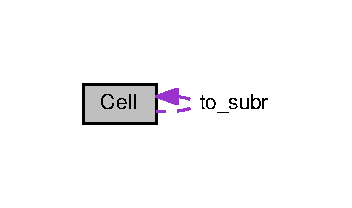
\includegraphics[width=169pt]{classCell__coll__graph}
\end{center}
\end{figure}
\subsection*{Public Member Functions}
\begin{DoxyCompactItemize}
\item 
\hypertarget{classCell_a3fc98c5b17b5136698f0d6cc5098d0b1}{bool {\bfseries is\-\_\-number} () const }\label{classCell_a3fc98c5b17b5136698f0d6cc5098d0b1}

\item 
\hypertarget{classCell_a2fa7c6bc8f1aaeea708987a458ee757d}{bool {\bfseries is\-\_\-string} () const }\label{classCell_a2fa7c6bc8f1aaeea708987a458ee757d}

\item 
\hypertarget{classCell_af65cb6ebca6eb0cdae92b94c6c9170eb}{bool {\bfseries is\-\_\-symbol} () const }\label{classCell_af65cb6ebca6eb0cdae92b94c6c9170eb}

\item 
\hypertarget{classCell_ad35f994b709c6f2d39c28d37ea531b5e}{bool {\bfseries is\-\_\-pair} () const }\label{classCell_ad35f994b709c6f2d39c28d37ea531b5e}

\item 
\hypertarget{classCell_aec416c3fd3e42f3f1561f0e4925ef079}{bool {\bfseries is\-\_\-frame} () const }\label{classCell_aec416c3fd3e42f3f1561f0e4925ef079}

\item 
\hypertarget{classCell_ac7e168b8aadf2f45d70edaa07cce1bcf}{bool {\bfseries is\-\_\-subr} () const }\label{classCell_ac7e168b8aadf2f45d70edaa07cce1bcf}

\item 
\hypertarget{classCell_a5feb82baf94f9ea40ab379ff40252057}{int {\bfseries to\-\_\-number} () const }\label{classCell_a5feb82baf94f9ea40ab379ff40252057}

\item 
\hypertarget{classCell_a07fffa139d78f90330cff5d2dec873a0}{string {\bfseries to\-\_\-string} () const }\label{classCell_a07fffa139d78f90330cff5d2dec873a0}

\item 
\hypertarget{classCell_a2b0c83446d5395274acd34bb1d749898}{string {\bfseries to\-\_\-symbol} () const }\label{classCell_a2b0c83446d5395274acd34bb1d749898}

\item 
\hypertarget{classCell_a28333096120ab2ee55f6b5349be1df3e}{\hyperlink{classCell}{Cell} $\ast$ {\bfseries to\-\_\-pair\-\_\-item} () const }\label{classCell_a28333096120ab2ee55f6b5349be1df3e}

\item 
\hypertarget{classCell_ae4b69fad453eabfef135575dfff784dc}{\hyperlink{classCell}{Cell} $\ast$ {\bfseries to\-\_\-pair\-\_\-next} () const }\label{classCell_ae4b69fad453eabfef135575dfff784dc}

\item 
\hypertarget{classCell_a5d07f221a15e84b35abe57071ea46cab}{\hyperlink{classFrame}{Frame} $\ast$ {\bfseries to\-\_\-frame} () const }\label{classCell_a5d07f221a15e84b35abe57071ea46cab}

\item 
\hypertarget{classCell_abb258fb7c184260fef5961f814bceb7f}{void {\bfseries make\-\_\-cell\-\_\-number} (int a)}\label{classCell_abb258fb7c184260fef5961f814bceb7f}

\item 
\hypertarget{classCell_ab0e4f4d88666cadc7d21a0cd3971efee}{void {\bfseries make\-\_\-cell\-\_\-string} (string s)}\label{classCell_ab0e4f4d88666cadc7d21a0cd3971efee}

\item 
\hypertarget{classCell_a56f50d1f105b2e8f087870f27d80e693}{void {\bfseries make\-\_\-cell\-\_\-symbol} (string s)}\label{classCell_a56f50d1f105b2e8f087870f27d80e693}

\item 
\hypertarget{classCell_a3ed1852893b5cdd81faa73e832451adf}{void {\bfseries make\-\_\-cell\-\_\-pair} (\hyperlink{classCell}{Cell} $\ast$p, \hyperlink{classCell}{Cell} $\ast$q)}\label{classCell_a3ed1852893b5cdd81faa73e832451adf}

\item 
\hypertarget{classCell_a437be131a0192328669af7539be7acb7}{void {\bfseries make\-\_\-cell\-\_\-frame} (\hyperlink{classFrame}{Frame} $\ast$f)}\label{classCell_a437be131a0192328669af7539be7acb7}

\item 
\hypertarget{classCell_a500fdba838de252002c7200ed863807c}{void {\bfseries make\-\_\-cell\-\_\-subr} (\hyperlink{classCell}{Cell} $\ast$($\ast$sub)(\hyperlink{classCell}{Cell} $\ast$lvals))}\label{classCell_a500fdba838de252002c7200ed863807c}

\end{DoxyCompactItemize}
\subsection*{Static Public Member Functions}
\begin{DoxyCompactItemize}
\item 
\hypertarget{classCell_aaddcdd9cbc00527042f0a67b07cf20e1}{static \hyperlink{classCell}{Cell} $\ast$ {\bfseries nil} ()}\label{classCell_aaddcdd9cbc00527042f0a67b07cf20e1}

\end{DoxyCompactItemize}
\subsection*{Public Attributes}
\begin{DoxyCompactItemize}
\item 
\hypertarget{classCell_afb40fe5500f4e871d2a5ea82afd3dbf4}{\hyperlink{classCell}{Cell} $\ast$($\ast$)(\hyperlink{classCell}{Cell} $\ast$) {\bfseries to\-\_\-subr} ()}\label{classCell_afb40fe5500f4e871d2a5ea82afd3dbf4}

\end{DoxyCompactItemize}


The documentation for this class was generated from the following files\-:\begin{DoxyCompactItemize}
\item 
cell.\-hh\item 
\hyperlink{cell_8cc}{cell.\-cc}\end{DoxyCompactItemize}

\hypertarget{classContinue__Directive}{\section{Continue\-\_\-\-Directive Class Reference}
\label{classContinue__Directive}\index{Continue\-\_\-\-Directive@{Continue\-\_\-\-Directive}}
}


{\ttfamily \#include $<$exception.\-hh$>$}

Inheritance diagram for Continue\-\_\-\-Directive\-:\begin{figure}[H]
\begin{center}
\leavevmode
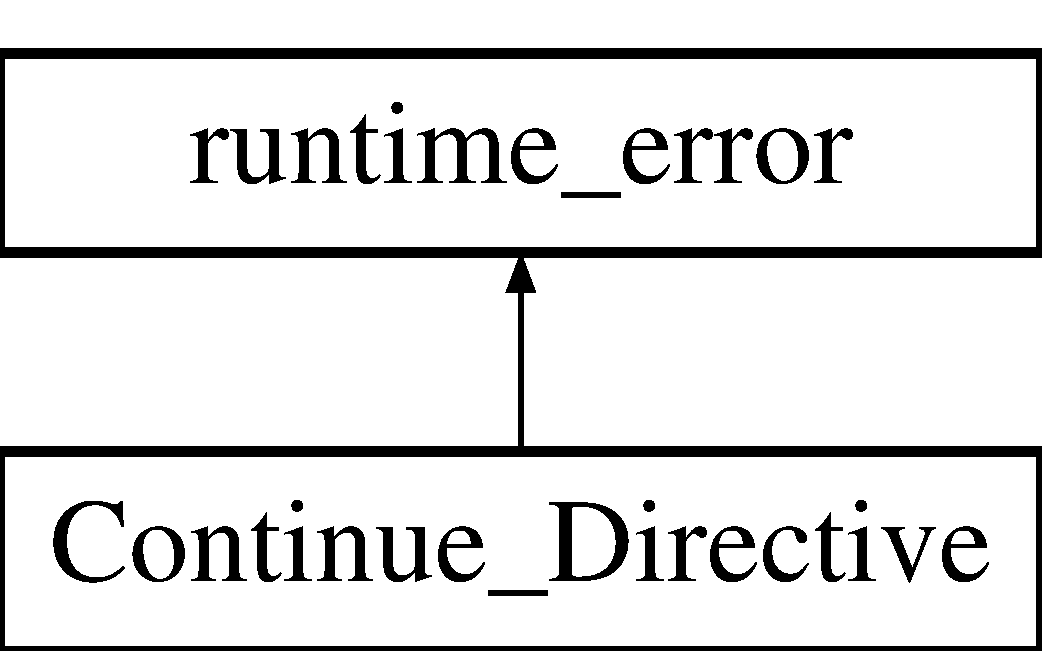
\includegraphics[height=2.000000cm]{classContinue__Directive}
\end{center}
\end{figure}


\subsection{Detailed Description}
toplevel exceptions 

The documentation for this class was generated from the following file\-:\begin{DoxyCompactItemize}
\item 
exception.\-hh\end{DoxyCompactItemize}

\hypertarget{classEnvBlock}{\section{Env\-Block Class Reference}
\label{classEnvBlock}\index{Env\-Block@{Env\-Block}}
}
\subsection*{Public Member Functions}
\begin{DoxyCompactItemize}
\item 
\hyperlink{classEnvBlock_a578ffa8ebc0161e6ec1bd014206de10f}{Env\-Block} ()
\item 
\hyperlink{classEnvBlock_a0158ee57b867427a39b8395af13629eb}{Env\-Block} (\hyperlink{classBinding}{Binding} cont, \hyperlink{classEnvBlock}{Env\-Block} $\ast$nex)
\item 
\hypertarget{classEnvBlock_a0860a0760290ddc69bdf14f766660c0c}{\hyperlink{classBinding}{Binding} $\ast$ {\bfseries get\-\_\-content} ()}\label{classEnvBlock_a0860a0760290ddc69bdf14f766660c0c}

\item 
\hypertarget{classEnvBlock_a03c712b1a137883e0ae303593c4c5e71}{\hyperlink{classEnvBlock}{Env\-Block} $\ast$ {\bfseries get\-\_\-next} ()}\label{classEnvBlock_a03c712b1a137883e0ae303593c4c5e71}

\item 
\hypertarget{classEnvBlock_a9c3c8875eca72db1bf042f9de83db78b}{void {\bfseries set\-\_\-next} (\hyperlink{classEnvBlock}{Env\-Block} $\ast$nex)}\label{classEnvBlock_a9c3c8875eca72db1bf042f9de83db78b}

\end{DoxyCompactItemize}


\subsection{Constructor \& Destructor Documentation}
\hypertarget{classEnvBlock_a578ffa8ebc0161e6ec1bd014206de10f}{\index{Env\-Block@{Env\-Block}!Env\-Block@{Env\-Block}}
\index{Env\-Block@{Env\-Block}!EnvBlock@{Env\-Block}}
\subsubsection[{Env\-Block}]{\setlength{\rightskip}{0pt plus 5cm}Env\-Block\-::\-Env\-Block (
\begin{DoxyParamCaption}
{}
\end{DoxyParamCaption}
)}}\label{classEnvBlock_a578ffa8ebc0161e6ec1bd014206de10f}
Creates an \hyperlink{classEnvBlock}{Env\-Block} containing a token binding \hypertarget{classEnvBlock_a0158ee57b867427a39b8395af13629eb}{\index{Env\-Block@{Env\-Block}!Env\-Block@{Env\-Block}}
\index{Env\-Block@{Env\-Block}!EnvBlock@{Env\-Block}}
\subsubsection[{Env\-Block}]{\setlength{\rightskip}{0pt plus 5cm}Env\-Block\-::\-Env\-Block (
\begin{DoxyParamCaption}
\item[{{\bf Binding}}]{cont, }
\item[{{\bf Env\-Block} $\ast$}]{nex}
\end{DoxyParamCaption}
)}}\label{classEnvBlock_a0158ee57b867427a39b8395af13629eb}
Creates an \hyperlink{classEnvBlock}{Env\-Block} containing the binding of cont to nex 

The documentation for this class was generated from the following files\-:\begin{DoxyCompactItemize}
\item 
env.\-hh\item 
env.\-cc\end{DoxyCompactItemize}

\hypertarget{classEnvironment}{\section{Environment Class Reference}
\label{classEnvironment}\index{Environment@{Environment}}
}
\subsection*{Public Member Functions}
\begin{DoxyCompactItemize}
\item 
\hypertarget{classEnvironment_acdb77ec0b3bc9b6b48ce430a8ff8d16d}{{\bfseries Environment} (\hyperlink{classFrame}{Frame} $\ast$obs)}\label{classEnvironment_acdb77ec0b3bc9b6b48ce430a8ff8d16d}

\item 
\hypertarget{classEnvironment_a73a2cb3642111c86485f48e70e5e4870}{\hyperlink{classFrame}{Frame} $\ast$ {\bfseries get\-\_\-observing} ()}\label{classEnvironment_a73a2cb3642111c86485f48e70e5e4870}

\item 
\hypertarget{classEnvironment_adac8db22e668d2a78a2cc18d0528c396}{void {\bfseries set\-\_\-new\-\_\-binding} (string name, \hyperlink{classCell}{Object} value)}\label{classEnvironment_adac8db22e668d2a78a2cc18d0528c396}

\item 
\hypertarget{classEnvironment_aaa7f24d4804dd8e2e9e95506b7c5bf58}{void {\bfseries add\-\_\-new\-\_\-binding} (string name, \hyperlink{classCell}{Object} value)}\label{classEnvironment_aaa7f24d4804dd8e2e9e95506b7c5bf58}

\item 
\hypertarget{classEnvironment_a29feed86a6e592d20f8c8882fcd35d6c}{void {\bfseries extend\-\_\-env} (\hyperlink{classCell}{Object} lpars, \hyperlink{classCell}{Object} lvals)}\label{classEnvironment_a29feed86a6e592d20f8c8882fcd35d6c}

\item 
\hypertarget{classEnvironment_aaa0fcf257cf27f961e51a9602cc2cb48}{\hyperlink{classCell}{Object} {\bfseries find\-\_\-value} (string name)}\label{classEnvironment_aaa0fcf257cf27f961e51a9602cc2cb48}

\item 
\hypertarget{classEnvironment_a61952d5ef784bff91ce1a66d6a00dc99}{void {\bfseries print} (ostream \&s)}\label{classEnvironment_a61952d5ef784bff91ce1a66d6a00dc99}

\item 
\hypertarget{classEnvironment_ace71e43a313cdeefb1e445ecef61825b}{\hyperlink{classCell}{Object} {\bfseries to\-\_\-\-Object} ()}\label{classEnvironment_ace71e43a313cdeefb1e445ecef61825b}

\item 
\hypertarget{classEnvironment_a852ae1aa43ba278c27a91e8dcc968086}{\hyperlink{classCell}{Object} {\bfseries make\-\_\-closure} (\hyperlink{classCell}{Object} body)}\label{classEnvironment_a852ae1aa43ba278c27a91e8dcc968086}

\end{DoxyCompactItemize}


The documentation for this class was generated from the following files\-:\begin{DoxyCompactItemize}
\item 
env.\-hh\item 
env.\-cc\end{DoxyCompactItemize}

\hypertarget{classEvaluation__Exception}{\section{Evaluation\-\_\-\-Exception Class Reference}
\label{classEvaluation__Exception}\index{Evaluation\-\_\-\-Exception@{Evaluation\-\_\-\-Exception}}
}


{\ttfamily \#include $<$exception.\-hh$>$}



Inheritance diagram for Evaluation\-\_\-\-Exception\-:\nopagebreak
\begin{figure}[H]
\begin{center}
\leavevmode
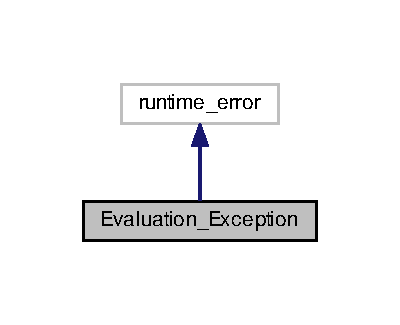
\includegraphics[width=192pt]{classEvaluation__Exception__inherit__graph}
\end{center}
\end{figure}


Collaboration diagram for Evaluation\-\_\-\-Exception\-:\nopagebreak
\begin{figure}[H]
\begin{center}
\leavevmode
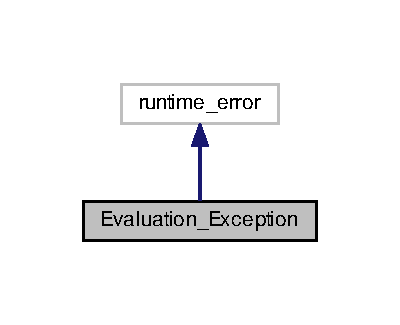
\includegraphics[width=192pt]{classEvaluation__Exception__coll__graph}
\end{center}
\end{figure}
\subsection*{Public Member Functions}
\begin{DoxyCompactItemize}
\item 
\hypertarget{classEvaluation__Exception_af7d73fddff98cbc5d503b18be20582f9}{{\bfseries Evaluation\-\_\-\-Exception} (\hyperlink{classCell}{Object} \-\_\-obj, \hyperlink{classEnvironment}{Environment} \-\_\-env, string \-\_\-message)}\label{classEvaluation__Exception_af7d73fddff98cbc5d503b18be20582f9}

\end{DoxyCompactItemize}


\subsection{Detailed Description}
Eval exceptions 

The documentation for this class was generated from the following file\-:\begin{DoxyCompactItemize}
\item 
\hyperlink{exception_8hh}{exception.\-hh}\end{DoxyCompactItemize}

\hypertarget{classFrame}{\section{Frame Class Reference}
\label{classFrame}\index{Frame@{Frame}}
}
\subsection*{Public Member Functions}
\begin{DoxyCompactItemize}
\item 
\hypertarget{classFrame_ad6270328988c4bf73df7f24a0e7cf5f7}{{\bfseries Frame} (\hyperlink{classFrame}{Frame} $\ast$\-\_\-scope)}\label{classFrame_ad6270328988c4bf73df7f24a0e7cf5f7}

\item 
\hypertarget{classFrame_a57eb3325f3ef059d1cab3ddb35e2a4ec}{{\bfseries Frame} (const \hyperlink{classFrame}{Frame} \&source)}\label{classFrame_a57eb3325f3ef059d1cab3ddb35e2a4ec}

\item 
\hypertarget{classFrame_aef63d90c2cd48dec6ac9b6dfd6f7d958}{void {\bfseries add\-\_\-new\-\_\-binding} (string name, \hyperlink{classCell}{Object} value)}\label{classFrame_aef63d90c2cd48dec6ac9b6dfd6f7d958}

\item 
\hypertarget{classFrame_a258655c409c6055a761ac8cc12fb2948}{void {\bfseries set\-\_\-new\-\_\-binding} (string name, \hyperlink{classCell}{Object} value)}\label{classFrame_a258655c409c6055a761ac8cc12fb2948}

\item 
\hypertarget{classFrame_a60853a5572534d23b5cf480c6217b9b8}{void {\bfseries extend\-\_\-env} (\hyperlink{classCell}{Object} lpars, \hyperlink{classCell}{Object} lvals)}\label{classFrame_a60853a5572534d23b5cf480c6217b9b8}

\item 
\hypertarget{classFrame_abe6a8a4589d130373c89147b660de034}{\hyperlink{classEnvBlock}{Env\-Block} $\ast$ {\bfseries find\-\_\-block} (string name)}\label{classFrame_abe6a8a4589d130373c89147b660de034}

\item 
\hypertarget{classFrame_a148a624be2406df10c0655c9d87d0544}{\hyperlink{classCell}{Object} {\bfseries find\-\_\-value} (string name)}\label{classFrame_a148a624be2406df10c0655c9d87d0544}

\item 
\hypertarget{classFrame_a5b0bcbaf2acba4166d94269a9b938834}{void {\bfseries print} (ostream \&s)}\label{classFrame_a5b0bcbaf2acba4166d94269a9b938834}

\end{DoxyCompactItemize}


The documentation for this class was generated from the following files\-:\begin{DoxyCompactItemize}
\item 
env.\-hh\item 
env.\-cc\end{DoxyCompactItemize}

\hypertarget{classNo__Binding__Exception}{\section{No\-\_\-\-Binding\-\_\-\-Exception Class Reference}
\label{classNo__Binding__Exception}\index{No\-\_\-\-Binding\-\_\-\-Exception@{No\-\_\-\-Binding\-\_\-\-Exception}}
}


{\ttfamily \#include $<$exception.\-hh$>$}



Inheritance diagram for No\-\_\-\-Binding\-\_\-\-Exception\-:\nopagebreak
\begin{figure}[H]
\begin{center}
\leavevmode
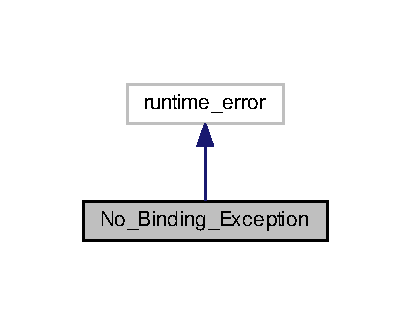
\includegraphics[width=197pt]{classNo__Binding__Exception__inherit__graph}
\end{center}
\end{figure}


Collaboration diagram for No\-\_\-\-Binding\-\_\-\-Exception\-:\nopagebreak
\begin{figure}[H]
\begin{center}
\leavevmode
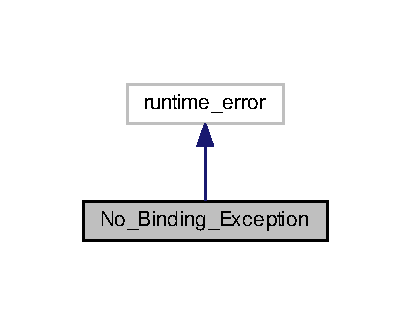
\includegraphics[width=197pt]{classNo__Binding__Exception__coll__graph}
\end{center}
\end{figure}
\subsection*{Public Member Functions}
\begin{DoxyCompactItemize}
\item 
\hypertarget{classNo__Binding__Exception_a83b63c7e8934d48a3a9476b75552e010}{{\bfseries No\-\_\-\-Binding\-\_\-\-Exception} (string \-\_\-name)}\label{classNo__Binding__Exception_a83b63c7e8934d48a3a9476b75552e010}

\end{DoxyCompactItemize}


\subsection{Detailed Description}
\hyperlink{classEnvironment}{Environment} Exceptions 

The documentation for this class was generated from the following file\-:\begin{DoxyCompactItemize}
\item 
\hyperlink{exception_8hh}{exception.\-hh}\end{DoxyCompactItemize}

\hypertarget{classNot__Subr}{\section{Not\-\_\-\-Subr Class Reference}
\label{classNot__Subr}\index{Not\-\_\-\-Subr@{Not\-\_\-\-Subr}}
}


{\ttfamily \#include $<$exception.\-hh$>$}

Inheritance diagram for Not\-\_\-\-Subr\-:\begin{figure}[H]
\begin{center}
\leavevmode
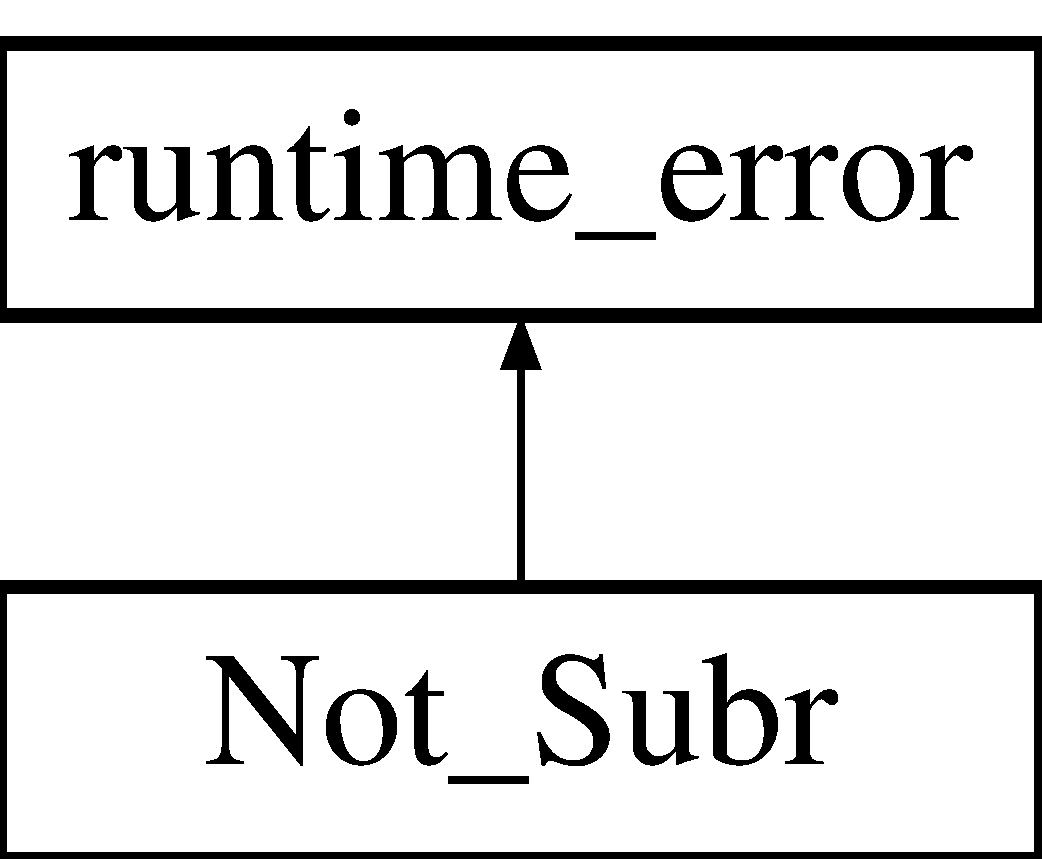
\includegraphics[height=2.000000cm]{classNot__Subr}
\end{center}
\end{figure}


\subsection{Detailed Description}
Subr exceptions 

The documentation for this class was generated from the following file\-:\begin{DoxyCompactItemize}
\item 
exception.\-hh\end{DoxyCompactItemize}

\hypertarget{structyy__buffer__state}{\section{yy\-\_\-buffer\-\_\-state Struct Reference}
\label{structyy__buffer__state}\index{yy\-\_\-buffer\-\_\-state@{yy\-\_\-buffer\-\_\-state}}
}
\subsection*{Public Attributes}
\begin{DoxyCompactItemize}
\item 
\hypertarget{structyy__buffer__state_a4843d1422e3276b636d475a3095bd948}{F\-I\-L\-E $\ast$ {\bfseries yy\-\_\-input\-\_\-file}}\label{structyy__buffer__state_a4843d1422e3276b636d475a3095bd948}

\item 
\hypertarget{structyy__buffer__state_ad7b8df8d8a4688e57b0b8d3ca75adc85}{char $\ast$ {\bfseries yy\-\_\-ch\-\_\-buf}}\label{structyy__buffer__state_ad7b8df8d8a4688e57b0b8d3ca75adc85}

\item 
\hypertarget{structyy__buffer__state_a58aa927f098b99d99e75da80f9b681ef}{char $\ast$ {\bfseries yy\-\_\-buf\-\_\-pos}}\label{structyy__buffer__state_a58aa927f098b99d99e75da80f9b681ef}

\item 
\hypertarget{structyy__buffer__state_a48302f5f3477a9c78bbddf56d356ef54}{yy\-\_\-size\-\_\-t {\bfseries yy\-\_\-buf\-\_\-size}}\label{structyy__buffer__state_a48302f5f3477a9c78bbddf56d356ef54}

\item 
\hypertarget{structyy__buffer__state_afcc44872643f513e79b43c2b1f334a67}{yy\-\_\-size\-\_\-t {\bfseries yy\-\_\-n\-\_\-chars}}\label{structyy__buffer__state_afcc44872643f513e79b43c2b1f334a67}

\item 
\hypertarget{structyy__buffer__state_a80ce2431c70dc4f89ced487f18449465}{int {\bfseries yy\-\_\-is\-\_\-our\-\_\-buffer}}\label{structyy__buffer__state_a80ce2431c70dc4f89ced487f18449465}

\item 
\hypertarget{structyy__buffer__state_abf5c70eea75581b58c0ee7bd31b14490}{int {\bfseries yy\-\_\-is\-\_\-interactive}}\label{structyy__buffer__state_abf5c70eea75581b58c0ee7bd31b14490}

\item 
\hypertarget{structyy__buffer__state_a9d60c60af6e1a6f69de16871fd64f85f}{int {\bfseries yy\-\_\-at\-\_\-bol}}\label{structyy__buffer__state_a9d60c60af6e1a6f69de16871fd64f85f}

\item 
int \hyperlink{structyy__buffer__state_a818e94bc9c766e683c60df1e9fd01199}{yy\-\_\-bs\-\_\-lineno}
\item 
int \hyperlink{structyy__buffer__state_a10c4fcd8be759e6bf11e6d3e8cdb0307}{yy\-\_\-bs\-\_\-column}
\item 
\hypertarget{structyy__buffer__state_a63d2afbb1d79a3fc63df9e12626f827d}{int {\bfseries yy\-\_\-fill\-\_\-buffer}}\label{structyy__buffer__state_a63d2afbb1d79a3fc63df9e12626f827d}

\item 
\hypertarget{structyy__buffer__state_a70fd925d37a2f0454fbd0def675d106c}{int {\bfseries yy\-\_\-buffer\-\_\-status}}\label{structyy__buffer__state_a70fd925d37a2f0454fbd0def675d106c}

\end{DoxyCompactItemize}


\subsection{Member Data Documentation}
\hypertarget{structyy__buffer__state_a10c4fcd8be759e6bf11e6d3e8cdb0307}{\index{yy\-\_\-buffer\-\_\-state@{yy\-\_\-buffer\-\_\-state}!yy\-\_\-bs\-\_\-column@{yy\-\_\-bs\-\_\-column}}
\index{yy\-\_\-bs\-\_\-column@{yy\-\_\-bs\-\_\-column}!yy_buffer_state@{yy\-\_\-buffer\-\_\-state}}
\subsubsection[{yy\-\_\-bs\-\_\-column}]{\setlength{\rightskip}{0pt plus 5cm}int yy\-\_\-buffer\-\_\-state\-::yy\-\_\-bs\-\_\-column}}\label{structyy__buffer__state_a10c4fcd8be759e6bf11e6d3e8cdb0307}
The column count. \hypertarget{structyy__buffer__state_a818e94bc9c766e683c60df1e9fd01199}{\index{yy\-\_\-buffer\-\_\-state@{yy\-\_\-buffer\-\_\-state}!yy\-\_\-bs\-\_\-lineno@{yy\-\_\-bs\-\_\-lineno}}
\index{yy\-\_\-bs\-\_\-lineno@{yy\-\_\-bs\-\_\-lineno}!yy_buffer_state@{yy\-\_\-buffer\-\_\-state}}
\subsubsection[{yy\-\_\-bs\-\_\-lineno}]{\setlength{\rightskip}{0pt plus 5cm}int yy\-\_\-buffer\-\_\-state\-::yy\-\_\-bs\-\_\-lineno}}\label{structyy__buffer__state_a818e94bc9c766e683c60df1e9fd01199}
The line count. 

The documentation for this struct was generated from the following file\-:\begin{DoxyCompactItemize}
\item 
lisp\-\_\-lex.\-c\end{DoxyCompactItemize}

\hypertarget{structyy__trans__info}{\section{yy\-\_\-trans\-\_\-info Struct Reference}
\label{structyy__trans__info}\index{yy\-\_\-trans\-\_\-info@{yy\-\_\-trans\-\_\-info}}
}
\subsection*{Public Attributes}
\begin{DoxyCompactItemize}
\item 
\hypertarget{structyy__trans__info_a5c9f61e770deef50bd4e697310342fe9}{flex\-\_\-int32\-\_\-t {\bfseries yy\-\_\-verify}}\label{structyy__trans__info_a5c9f61e770deef50bd4e697310342fe9}

\item 
\hypertarget{structyy__trans__info_ae0715250c2bef261e596e77e0030f13e}{flex\-\_\-int32\-\_\-t {\bfseries yy\-\_\-nxt}}\label{structyy__trans__info_ae0715250c2bef261e596e77e0030f13e}

\end{DoxyCompactItemize}


The documentation for this struct was generated from the following file\-:\begin{DoxyCompactItemize}
\item 
lisp\-\_\-lex.\-c\end{DoxyCompactItemize}

\hypertarget{unionyyalloc}{\section{yyalloc Union Reference}
\label{unionyyalloc}\index{yyalloc@{yyalloc}}
}
\subsection*{Public Attributes}
\begin{DoxyCompactItemize}
\item 
\hypertarget{unionyyalloc_a4800e0520a89a4789afa7b5d82197e65}{yytype\-\_\-int16 {\bfseries yyss\-\_\-alloc}}\label{unionyyalloc_a4800e0520a89a4789afa7b5d82197e65}

\item 
\hypertarget{unionyyalloc_a9326f4fdc6f737a929444427836d8928}{\hyperlink{unionYYSTYPE}{Y\-Y\-S\-T\-Y\-P\-E} {\bfseries yyvs\-\_\-alloc}}\label{unionyyalloc_a9326f4fdc6f737a929444427836d8928}

\end{DoxyCompactItemize}


The documentation for this union was generated from the following file\-:\begin{DoxyCompactItemize}
\item 
lisp\-\_\-yacc.\-c\end{DoxyCompactItemize}

\hypertarget{unionYYSTYPE}{\section{Y\-Y\-S\-T\-Y\-P\-E Union Reference}
\label{unionYYSTYPE}\index{Y\-Y\-S\-T\-Y\-P\-E@{Y\-Y\-S\-T\-Y\-P\-E}}
}
\subsection*{Public Attributes}
\begin{DoxyCompactItemize}
\item 
\hypertarget{unionYYSTYPE_ad89069baa0a35ece66a52b315835abe6}{\hyperlink{classCell}{Object} {\bfseries Object\-\_\-value}}\label{unionYYSTYPE_ad89069baa0a35ece66a52b315835abe6}

\item 
\hypertarget{unionYYSTYPE_a85e325a8c56800cb3c763fb0aae89b28}{int {\bfseries number\-\_\-value}}\label{unionYYSTYPE_a85e325a8c56800cb3c763fb0aae89b28}

\item 
\hypertarget{unionYYSTYPE_ac01a27ce7f2f4974d8b55b4ba00429a0}{char $\ast$ {\bfseries string\-\_\-value}}\label{unionYYSTYPE_ac01a27ce7f2f4974d8b55b4ba00429a0}

\end{DoxyCompactItemize}


The documentation for this union was generated from the following files\-:\begin{DoxyCompactItemize}
\item 
lisp\-\_\-yacc.\-c\item 
lisp\-\_\-yacc.\-h\end{DoxyCompactItemize}

\hypertarget{classZipping__Exception}{\section{Zipping\-\_\-\-Exception Class Reference}
\label{classZipping__Exception}\index{Zipping\-\_\-\-Exception@{Zipping\-\_\-\-Exception}}
}
Inheritance diagram for Zipping\-\_\-\-Exception\-:\begin{figure}[H]
\begin{center}
\leavevmode
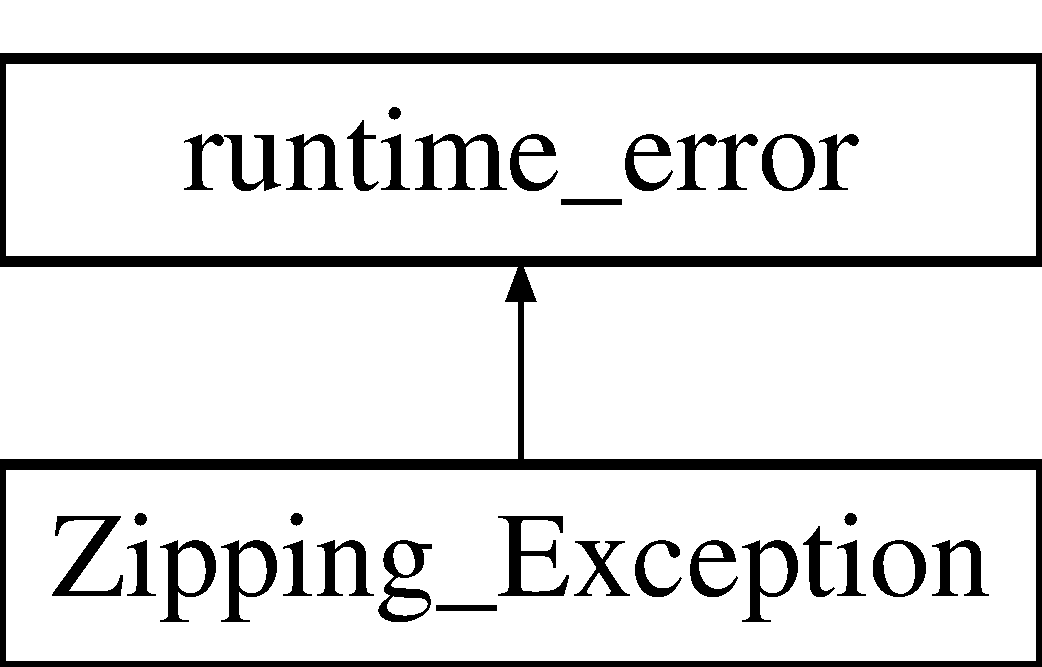
\includegraphics[height=2.000000cm]{classZipping__Exception}
\end{center}
\end{figure}
\subsection*{Public Member Functions}
\begin{DoxyCompactItemize}
\item 
\hypertarget{classZipping__Exception_a7ea62c850ba54f7644f156dcb7c21826}{{\bfseries Zipping\-\_\-\-Exception} (\hyperlink{classCell}{Object} \-\_\-lobjs, string \-\_\-message)}\label{classZipping__Exception_a7ea62c850ba54f7644f156dcb7c21826}

\end{DoxyCompactItemize}


The documentation for this class was generated from the following file\-:\begin{DoxyCompactItemize}
\item 
exception.\-hh\end{DoxyCompactItemize}

%--- End generated contents ---

% Index
\newpage
\phantomsection
\addcontentsline{toc}{chapter}{Index}
\printindex

\end{document}
